\subsection{Overview}
    \begin{frame}
        \frametitle{Overview}
        \visible<1->{In this defense, I will show that I successfully:} 
        \begin{enumerate}
            \visible<2->{\item Furthered our understanding of the \gls{AHTR} design's 
            complexities through neutronics and temperature modeling}
            \visible<3->{\item Created an open-source tool that enables reactor generative 
            design optimization with evolutionary algorithms}
            \visible<4->{\item Applied the optimization tool to the \gls{AHTR} design for 
            non-conventional geometries and fuel distributions} 
        \end{enumerate}
    \end{frame}

\subsection{Background: Advanced High Temperature Reactor}
    \begin{frame}
        \frametitle{MSR + VHTR = FHR}
        \visible<1-3>{Gen IV Forum identified \textbf{new and innovative Gen IV nuclear energy systems}: 
        Molten Salt Reactors (MSR) and Very High-Temperature Reactors (VHTR).} 
        \vspace{0.2cm}
        \begin{columns}
        \visible<2-3>{\begin{column}{0.5\textwidth}

        \vspace{-0.1cm}
        The \textbf{Fluoride-Salt Cooled High-Temperature Reactor (FHR) concept 
        combines the best aspects of MSR and VHTR}.

        The \acrfull{AHTR} is a subset of the FHR. 
        \vspace{-0.6cm}
        \begin{figure}[]
                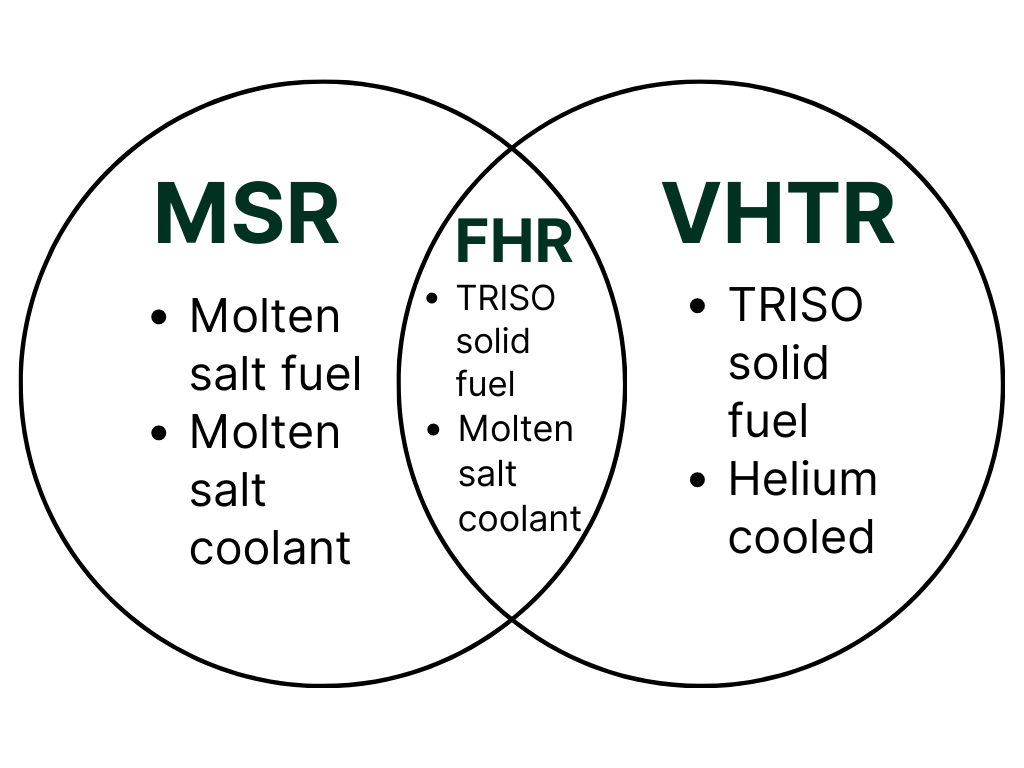
\includegraphics[width=0.95\linewidth]{figures/fhr_venn.png}
            %\caption{FHR Venn diagram.}
        \end{figure}
        \end{column}}
        \visible<3>{
        \begin{column}{0.5\textwidth}

            \vspace{-0.15cm}
            \acrfull{FLiBe} salt cooled: \textbf{superior cooling, low operating 
            pressure}
            
            \vspace{0.1cm}
            \acrfull{TRISO} fuel: fuel kernel encapsulated in three other layers, 
            \textbf{extra barriers to fission product release, higher safety margin} 
            \vspace{-0.1cm}
            \begin{figure}[htbp!]
                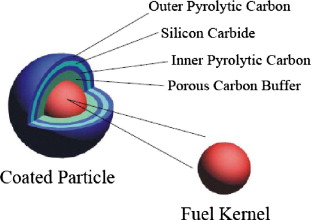
\includegraphics[width=0.6\linewidth]{figures/triso.png}
                \caption{TRISO diameter $\approx 8mm$.}
            \end{figure}
        \end{column}}
    \end{columns}
        \end{frame}

    \begin{frame}
    \frametitle{Advanced High Temperature Reactor Design}
        \begin{itemize}
        \item Design developed by Oak Ridge National Laboratory
        \item Prismatic FHR design with 252 hexagonal fuel assemblies consisting of 
        18 fuel planks arranged in 3 diamond-shaped sectors
        \end{itemize}
    
    \vspace{0.2cm}
    \begin{figure}[]
        \centering
        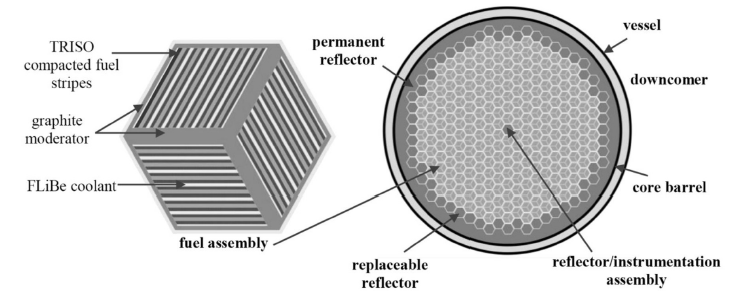
\includegraphics[width=\linewidth]{../docs/figures/ahtr.png} 
        \caption{\acrlong{AHTR} full assembly (left) and core configuration (right) 
        reproduced from \cite{ramey_monte_2018}.}
        \label{fig:ahtr}
    \end{figure}
    \end{frame}

    \begin{frame}
    \frametitle{Advanced High Temperature Reactor Geometry}
    \visible<1->{\begin{figure}[]
        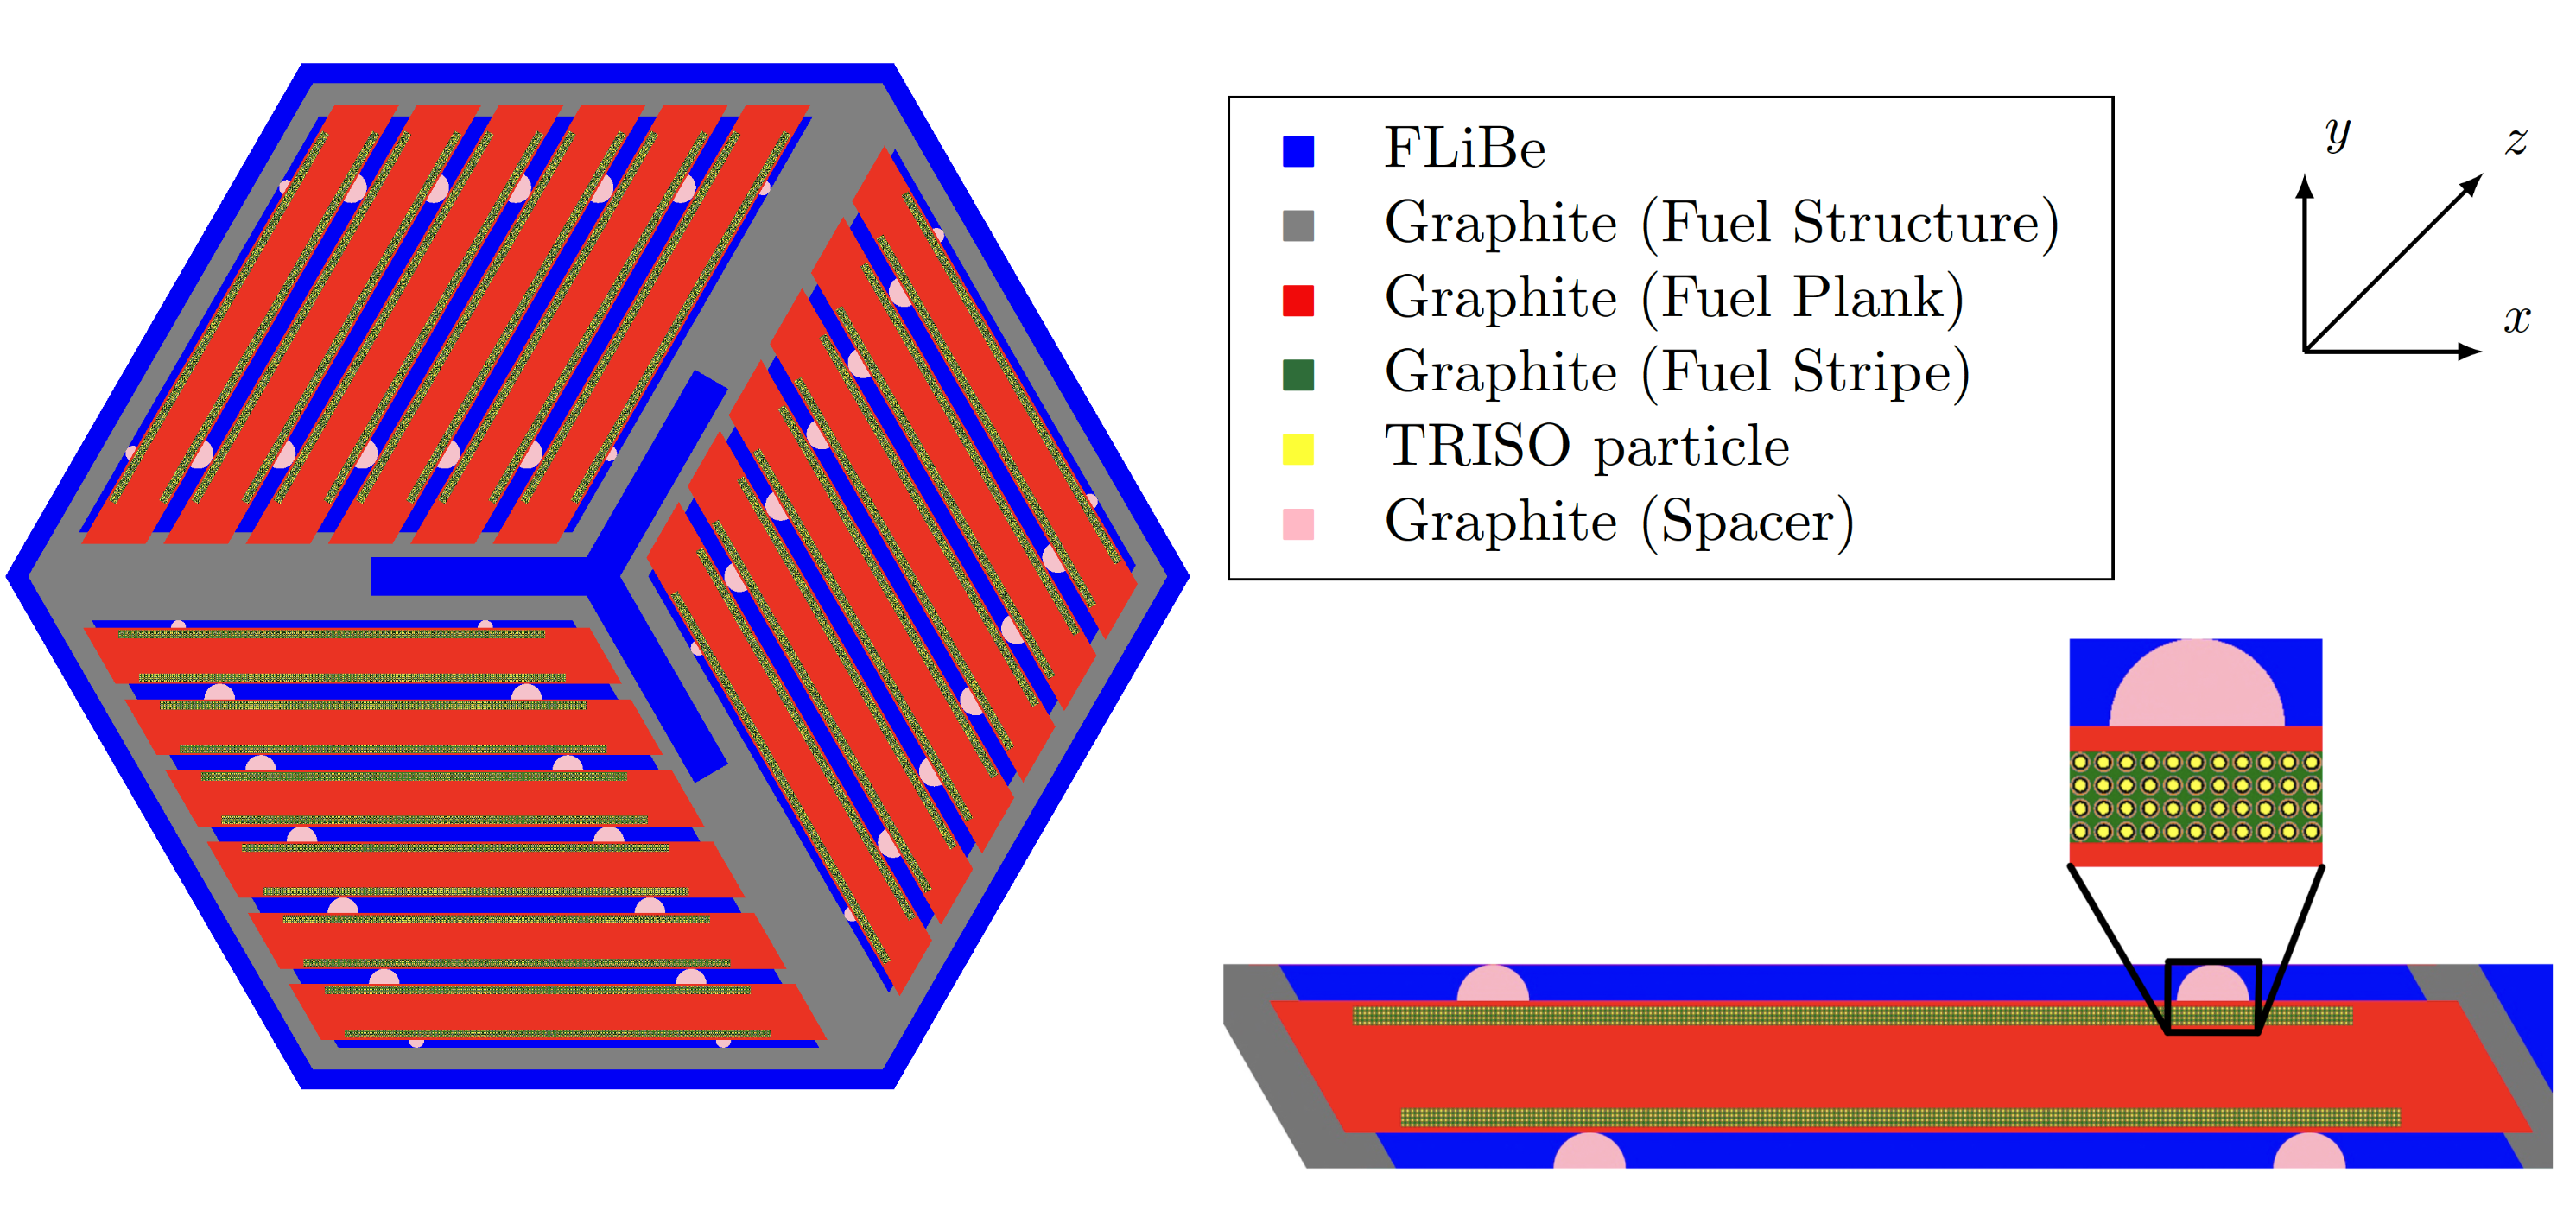
\includegraphics[width=0.95\linewidth]{figures/ahtr-assembly.png} 
        \caption{AHTR full assembly with 18 fuel plates arranged in 
        three diamond-shaped sectors, with a central Y-shaped and external channel 
        graphite structure.}
    \end{figure}}
    \vspace{-0.2cm}
    \visible<2->{The AHTR has \textbf{triple heterogeneity}: hexagonal fuel 
    elements within the core, and TRISO particles embedded in stripes within each plank.}
    \end{frame}

    \begin{frame}
    \frametitle{FHR Benchmark}
    \visible<1->{The AHTR's geometry's triple heterogeneity results in
    \textbf{complex reactor physics} and \textbf{significant modeling challenges}.}
    \begin{itemize}
        \item Many surfaces to model = computationally expensive
        \item Homogenization might result in loss of reactor physics effects
    \end{itemize}
    \vspace{0.3cm}
    \visible<2->{In 2019 the \textbf{OECD-NEA initiated the FHR benchmark}. Its objective 
    is to identify the applicability, accuracy, and practicality of the latest 
    methods and codes to assess the current state of the art for FHR modeling.

    \vspace{0.2cm}
    \begin{figure}[]
        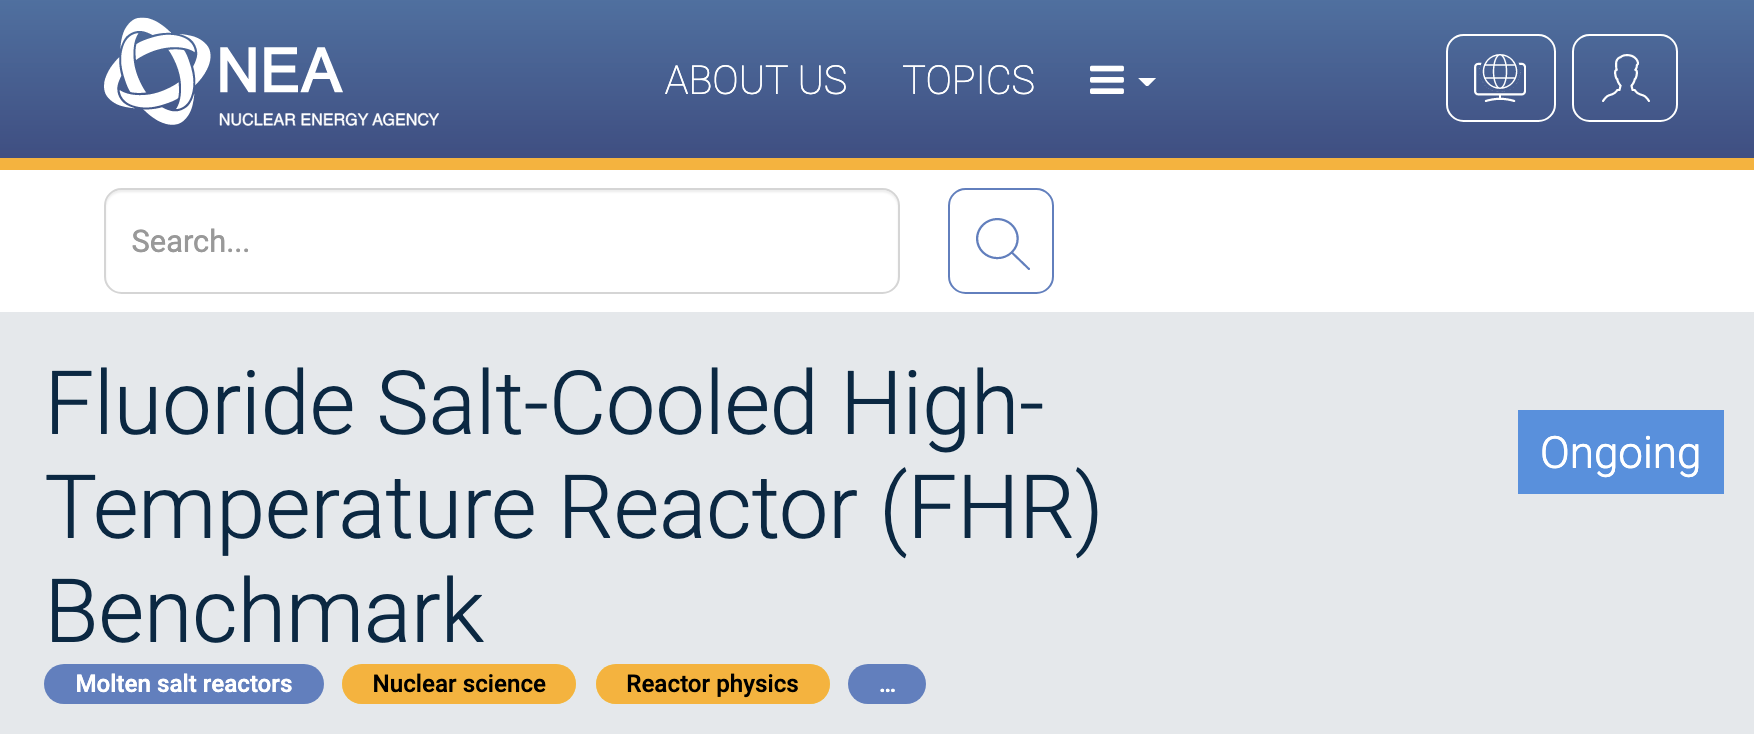
\includegraphics[width=0.7\linewidth]{figures/benchmark.png} 
        \caption{OECD NEA's FHR Benchmark \cite{petrovic_benchmark_2021}.}
    \end{figure}}
    \end{frame}

\subsection{Objectives: AHTR Model Development}
    \begin{frame}
        \frametitle{Research Objectives: AHTR Model Development}
        \visible<1->{\begin{block}{Technical Gap}
            The geometrically complex AHTR design is challenging to model accurately 
            and computationally expensive. 
        \end{block}}
        \visible<2->{\begin{block}{Research Objectives: AHTR Model Development}
        \begin{itemize}
            \item Participate in FHR benchmark's neutronics modeling to further our 
            understanding of the AHTR design's complexities
            \item AHTR temperature model to capture thermal feedback effects
        \end{itemize}
        \end{block}}
        \visible<3->{\begin{block}{Link to Reactor Optimization for Non-conventional Designs}
        \begin{itemize}
        \item By participating in the benchmark, I ensure an accurate AHTR base model
        \item Thus, I can expect accurate answers for the optimized AHTR designs
        \end{itemize}
        \end{block}}
    \end{frame}

\subsection{Background: Generative Reactor Design Optimization}
\begin{frame}
    \frametitle{Overview}
    In this defense, I will show that I successfully: 
    \begin{enumerate}
        \item Furthered our understanding of the \gls{AHTR} design's complexities 
        through neutronics and temperature modeling
        \item Created an open-source tool that enables reactor generative 
        design optimization with evolutionary algorithms
        \item Applied the optimization tool to the \gls{AHTR} design for 
        non-conventional geometries and fuel distributions 
    \end{enumerate}
\end{frame}

\begin{frame}
    \frametitle{3D Printing a Nuclear Reactor}
    \visible<1->{Additive manufacturing enables us to \textbf{surpass classical 
    manufacturing constraints} and optimize for \textbf{arbitrary geometries and 
    parameters}.} 
    \visible<2->{\begin{figure}[]
        \begin{minipage}[r]{0.45\textwidth}
            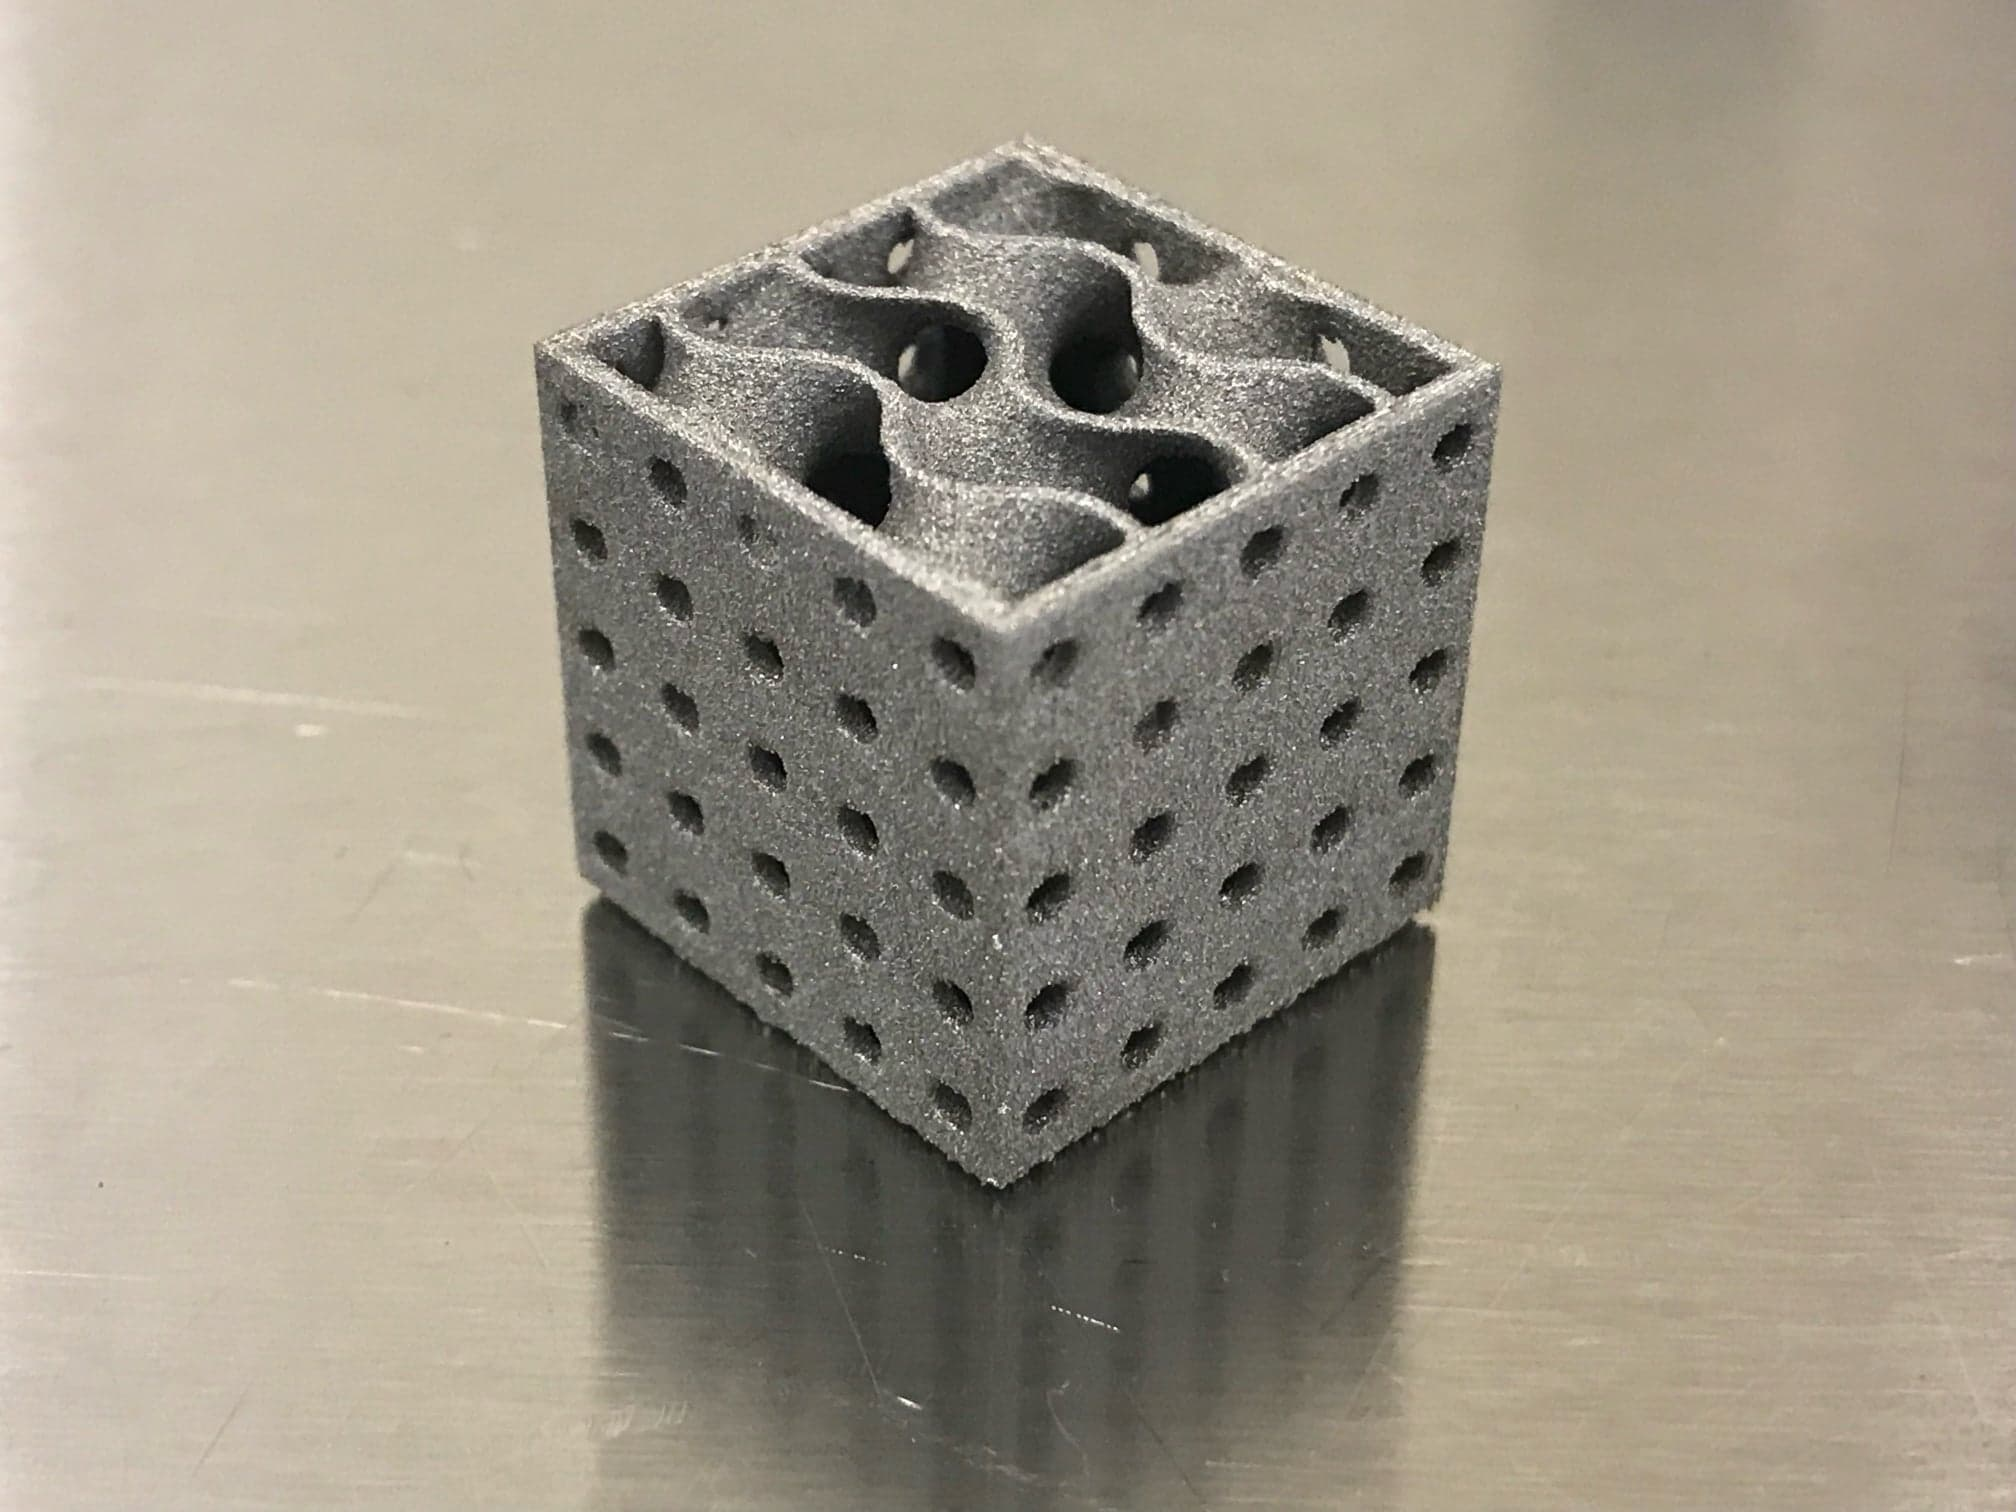
\includegraphics[width=0.7\linewidth]{figures/tungsten-wavy-channels.png}            
        \end{minipage}
        \begin{minipage}[l]{0.5\textwidth}
            \caption{3D printed Tungsten wavy flow channels, reproduced from NASA's Refractory 
            Alloy Additive Manufacturing Build Optimization Project (RAAMBO) 
            \cite{mireles_refractory_2022}.}        
        \end{minipage}
    \end{figure}}

    \visible<2->{Wide-spread adoption of 3D printing for reactor parts could \textbf{reduce 
    fabrication costs and deployment timelines, and improve reactor safety and 
    performance}.}

    \vspace{0.1cm}
    \visible<3->{We require methods, such as \textbf{generative design}, to explore the 
    new design space more efficiently.} 
\end{frame}

  \begin{frame}
    \frametitle{Generative Reactor Design Optimization}
    \visible<1->{Generative design is an \textbf{iterative design exploration process} 
    \cite{autodesk_autodesk_2020}. 
    \begin{itemize}
        \item Designers provide design goals and constraints to the generative design 
        software
        \item Software explores all the possible permutations of a solution, quickly generating 
        design alternatives
    \end{itemize}}

    \vspace{0.2cm}
    \visible<2->{The generative design software \textbf{automates the search process for 
    suitable geometries}. 

    \vspace{0.2cm}
    The human reactor designer can instead focus on 
    \begin{itemize}
        \item \textbf{Defining design criteria} for optimal designs 
        \item \textbf{Evaluating the results} generated by generative design software  
    \end{itemize}}

    \vspace{0.2cm}
    \visible<3->{\textbf{Evolutionary algorithms} can be used to \textbf{drive generative 
    reactor design optimization} to promptly explore the large design space to find 
    global optimal designs.}
  \end{frame}

    \begin{frame}
    \frametitle{Evolutionary Algorithms for Reactor Generative Design}
    \begin{minipage}{0.59\textwidth}
        \visible<1->{\textbf{Evolutionary Algorithms} 
        \begin{itemize}
            \item \textbf{Imitate natural selection} to evolve solutions 
            \item Uses simple mechanisms: \textbf{selection} (selects good 
            individuals), \textbf{mutation} and \textbf{crossover} (creates 
            better individuals)
            \item \textbf{Average population improves with every generation} 
        \end{itemize}}

        \visible<2->{Evolutionary Algorithm \textbf{Benefits} 
        \begin{itemize} 
            \item \textbf{Computationally simple}
            \item Proven to be successful at finding \textbf{globally optimal solutions} 
            for multi-objective optimization problems 
            \item Can take advantage of \textbf{parallel systems} 
        \end{itemize}}
        \end{minipage}
    \begin{minipage}[c]{0.4\textwidth}
        \visible<1->{\begin{figure}
                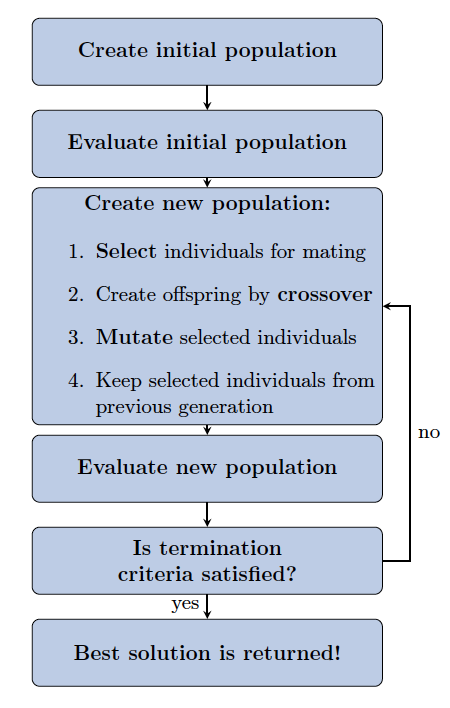
\includegraphics[width=\textwidth]{figures/ea-flow.png}
            %\caption{Evolutionary algorithm flow \cite{renner_genetic_2003}. }
          \end{figure}}
    \end{minipage}
    \end{frame}

\subsection{Objectives: AHTR Optimization for Non-Conventional Designs}
\begin{frame}
    \frametitle{Research Objectives: AHTR optimization for non-conventional designs}
    \visible<1->{\begin{block}{Technical Gap}
      \begin{itemize}
        \item Optimization tools for generating new reactor designs enabled by
        3D printing do not exist
        \item Few demonstrations of reactor optimization for non-conventional 
        geometries and parameters exist
      \end{itemize}
    \end{block}}
    \visible<2->{\begin{block}{Research Objectives: AHTR optimization for non-conventional designs}
        \begin{itemize}
            \item Develop an open-source tool that enables generative reactor design 
            optimization with evolutionary algorithms 
            \item Demonstrate successful tool application on AHTR optimization for 
            non-conventional reactor geometries and fuel distributions
        \end{itemize}
    \end{block}}
  \end{frame}

\subsection{Summary}
\begin{frame}
    \frametitle{Research Objectives Summary}
    \visible<1->{\begin{block}{Research Objectives: AHTR Model Development}
        \begin{itemize}
            \item Participate in the OECD-NEA's FHR Benchmark with OpenMC 
            \cite{romano_openmc:_2015}
            \item AHTR temperature model with Moltres \cite{lindsay_introduction_2018}
        \end{itemize}
    \end{block}}

    \visible<2->{\begin{block}{Research Objectives: AHTR optimization for non-conventional 
        designs}
        \begin{itemize}
            \item Develop an open-source tool that enables generative reactor design 
            optimization with evolutionary algorithms 
            \item Demonstrate successful tool application on AHTR optimization for 
            non-conventional reactor geometries and fuel distributions
        \end{itemize}
    \end{block}}
\end{frame}